\section{Resolución Problema 2} 
Dada una ecuación cuadrática regresar los valores de las raíces, en caso de que estén sobre el conjunto de números reales, en caso contrario indicar que la solución esta en el conjunto de los números complejos.


\subsection{\textbf{Descripción del problema:}}
El problema planteado se centra en la resolución de una ecuación cuadrática y la determinación de sus posibles soluciones. La ecuación cuadrática tiene la forma general $ax^{2}+bx+c$, donde a, b y c son los coeficientes dados. El objetivo es aplicar la fórmula general:
\begin{equation}
\\
\\ x = \frac{{-b \pm \sqrt{{b^2 - 4ac}}}}{{2a}} \\
\end{equation}
\\
\\Para obtener las soluciones de la ecuación.

Para determinar la naturaleza de las soluciones, se utiliza el discriminante, que está dado por la expresión 
\begin{equation}
 b^2 - 4ac 
\end{equation}
\\Dependiendo del valor del discriminante, se obtienen tres casos posibles:
\begin{itemize}
    \item Si el discriminante > 0 se dan dos soluciones
    \item Si el discriminante = 0 se da una solución
    \item Si el discriminante es < 0 la solución se encuentra en el conjunto de los números complejos. 
\end{itemize}
 Estos casos permiten clasificar las soluciones de la ecuación cuadrática en función de su naturaleza y son determinantes para comprender las propiedades y características de la ecuación en cuestión.


\begin{figure}[H]
    \centering
    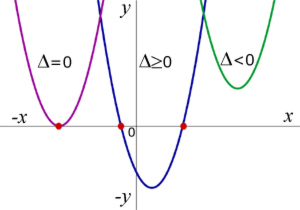
\includegraphics[width = 6 cm]{LaTeX/imagenes/discriminant.jpg}
    \caption{Discriminante}
    \label{fig:Discriminante}
\end{figure}


\subsection{\textbf{Definición de solución:}}
Se plantea la resolución de una ecuación cuadrática en la forma 
\begin{equation}
ax^{2}+bx+c
\end{equation}
donde se procede al cálculo del discriminante y a la evaluación de tres condiciones. En caso de que el discriminante sea mayor que cero, se llevan a cabo dos operaciones y se presenta el resultado correspondiente. Si el discriminante es igual a cero, se realiza una operación y se muestra el resultado obtenido. Por otro lado, si el discriminante resulta ser negativo, se informa al usuario que la ecuación en cuestión no cuenta con soluciones reales.

Acto seguido se muestra el diagrama de flujo, el cual es la base del programa.

\begin{figure}[H]
    \centering
    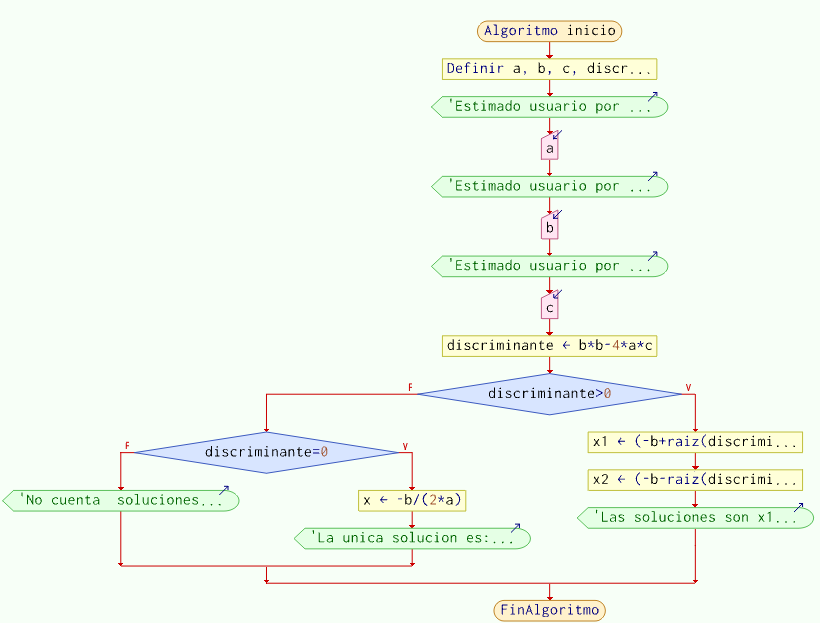
\includegraphics[width = 6 cm]{LaTeX/imagenes/Diagrama2.png}
    \caption{Diagrama de flujo}
    \label{fig:diagrama de flujo}
\end{figure}


\subsection{\textbf{Diseño de la solución:}}
Se plantea la resolución de una ecuación cuadrática en la forma 
\begin{equation}
ax^{2}+bx+c
\end{equation}
donde se procede al cálculo del discriminante y a la evaluación de tres condiciones. En caso de que el discriminante sea mayor que cero, se llevan a cabo dos operaciones y se presenta el resultado correspondiente. Si el discriminante es igual a cero, se realiza una operación y se muestra el resultado obtenido. Por otro lado, si el discriminante resulta ser negativo, se informa al usuario que la ecuación en cuestión no cuenta con soluciones reales.

Acto seguido se muestra el diagrama de flujo, el cual es la base del programa.

\begin{figure}[H]
    \centering
    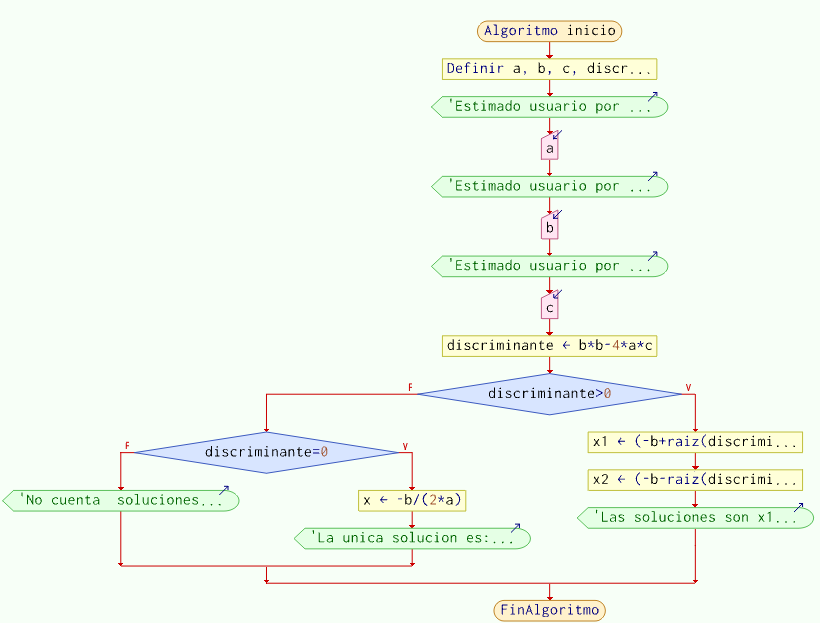
\includegraphics[width = 6 cm]{LaTeX/imagenes/Diagrama2.png}
    \caption{Diagrama de flujo}
    \label{fig:diagrama de flujo}
\end{figure}


\subsection{\textbf{Desarrollo de la solución:}}
eguidamente se mostrara el programa de java, donde se trabajo con la formula general. Para ello, se ocupan las librería Math y el objeto Scanner.
\begin{javaCode}
    
import java.util.Scanner;

    
        Crear un objeto Scanner para leer la entrada del usuario
        \begin{javaCode}
        Scanner coeficiente = new Scanner(System.in);
        \end{javaCode}
        Solicitar al usuario que ingrese el valor de A
        \begin{javaCode}
        System.out.println("Estimado usuario, por favor ingrese el valor de A: ");
        double a = coeficiente.nextDouble();
        \end{javaCode}
        Solicitar al usuario que ingrese el valor de B
        \begin{javaCode}
        System.out.println("Estimado usuario, por favor ingrese el valor de B: ");
        double b = coeficiente.nextDouble();
        \end{javaCode}
        Solicitar al usuario que ingrese el valor de C
        \begin{javaCode}
        System.out.println("Estimado usuario, por favor ingrese el valor de C: ");
        double c = coeficiente.nextDouble();
        \end{javaCode}
        Cierra el objeto Scanner
        \begin{javaCode}
        coeficiente.close();
        \end{javaCode}
        Calcula el discriminante de la ecuación cuadrática
        \begin{javaCode}
        double discriminante = b * b - 4 * a * c;
        \end{javaCode}
       El objetivo es verificar si el discriminante de una ecuación cuadrática es mayor que cero. Si se cumple esta condición, se determina que la ecuación tiene dos soluciones. Luego, se resuelven las soluciones y se muestra el resultado al usuario.
        \begin{javaCode}
        if (discriminante > 0) {
            double x1 = (-b + Math.sqrt(discriminante)) / (2 * a);
            double x2 = (-b - Math.sqrt(discriminante)) / (2 * a);
       
            System.out.println("Las soluciones son x1 = " + x1 + " y x2 = " + x2);
        }
        \end{javaCode}
        Verificar si el discriminante es igual a 0, si cumple con la condición, realiza la operación donde solo existe una única solución y la muestra al usuario
        \begin{javaCode}
        else if (discriminante == 0) 
           
            double x = -b / (2 * a);

            System.out.println("La solucion es: " + x);
        
        \end{javaCode}
        En caso de que el discriminante sea negativo, se determina que la ecuación cuadrática no tiene soluciones reales. Esta información se comunica al usuario.
        \begin{javaCode}
        else {
            System.out.println("no cuenta con soluciones reales.");
        }
    



\end{javaCode}



\subsection{\textbf{Depuración y pruebas:}}
del mismo. Donde se muestra los diferentes resultados posibles.
\begin{center}
\begin{tabular}{|c|c|c|c|c|}
\hline
No. & A & B & C & Resultado \\
\hline
1 & 19 & 17 & 18 & no cuenta con soluciones reales. \\
\hline
2 & 10 & 15 & 5 & La solución es:$x_1 = -0.5$ y $x_2=-1.0$ \\
\hline
3 & 1 & -2 & 1 & La solución es:$x=1 \\
\hline
4 & 2 & 4 & -6 &La solución es:$x_1 = 1.0$ y $x_2=-3.0$ \\
\hline
5 & 1 & 1 & 1 & No cuenta con soluciones reales. \\
\hline
\end{tabular}
\label{fig: Tabla de ejecución}
\end{center}